\section{Significance, Background, and Technical Approach}

RNET Technologies Inc. (RNET) in Dayton, OH and Oak Ridge National Laboratory 
(ORNL) are responding to the 2019 DOE SBIR/STTR Phase II Release 2 
(DE-FOA-0001976). This proposal is for a Phase II contract in succession to an 
initial Phase I contract (Contract \#: DE-SC0018728) awarded for DOE 
SBIR/STTR Topic 30d (Modeling and Simulation). Based on a prototype developed in Phase I, RNET and ORNL are proposing the development of VnV: a self-documenting testing framework for end-user solution verification and validation in high performance computing applications. This proposal will highlight the need for, and the tremendous value of, the proposed tool in high performance numerical simulations. The goal of the proposed Phase II project will be to develop and demonstrate a production quality implementation of the VnV framework that delivers this value across a broad spectrum of numerical applications. 

RNET has extensive SBIR experience in high performance computing, including performance optimization of numerical software and libraries, development of fine-grained power monitoring tools for HPC infrastructure, and the development of software usability tools that enhance the user experience. Dr. Watson, our collaborator at ORNL, is an experienced software professional with extensive knowledge of software design, architecture, and engineering practices. He has experience developing parallel debugging software for HPC environments and  is the project leader of the open-source Eclipse Parallel Tools Platform (PTP). We believe that our experience developing advanced numerical software for the HPC community combined with Dr. Watson's experience with scientific software engineering uniquely qualifies our team to develop and commercialize the VnV framework.

\subsection{Identification and Significance of the Innovation}
\label{sec:identification}
%% {\em Define the specific technical problem or opportunity addressed by
%%  your application.  Provide enough background information so that the
%%  importance of the problem/opportunity is clear.  Indicate the overall
%%  technical approach to the problem/opportunity and the part that the
%%  proposed research plays in providing needed results.}


\subsubsection{Identification and Significance}
\label{intro}
Numerical modeling and simulation (M\&S) is almost always more economical than live testing and prototyping; a fact that has seen wide-scale uptake in the R\&D life-cycles of products ranging from \$10 polycarbonate toys, up to solar panels, airplane wings and nuclear reactors. With access to high performance computational resources at an all time high, and with exascale computing resources on the horizon; the role \MS has in the design pipelines of next generation technologies is only expected to increase. However, numerical simulations are, by definition, an \emph{approximation} to a real world physical system. As such, it is important that this increased reliance on simulated tests is accompanied by a concerted effort to ensure simulations are fit for the intended purpose. As stated in the DoD best practices guide \cite{dodvv}, verification and validation (V\&V) of a code should be performed when  \emph{``...the risk of making an incorrect decision based on a simulation outweighs the time and cost of performing \VV to ensure that a simulation produces results that are sufficiently accurate and reliable.''} One only needs to look to the Sleipner platform accident, where an offshore oil platform collapsed due to failures in the finite element simulation, to get an idea of the devastating consequences poorly verified numerical simulations can have on business, the environment and society.

The staples of a rigorous \VV regimen are:

\begin{itemize}
 \item The development of a detailed \VV plan.
 \item The implementation of software development best practices (e.g. version control, unit and regression testing, code reviews, etc.).
 \item Mathematical and algorithmic testing (convergence analysis, mesh refinement studies, method of manufactured solutions, etc.).
 \item Development of a broad benchmark testing suite.
 \item Uncertainty quantification and sensitivity analysis.
 \item Comparison of simulation results with experimental data and results from third party simulations. 
 \item Review of the implementation and results by experts in the field.
 \item Documentation of the \VV effort.
\end{itemize}

\VV is a discrete process that cannot account for each and every possibility. This raises issues in the development of general purpose numerical simulation packages because, while it may be the developers responsibility to ensure the product is mathematically correct, it is ultimately the responsibility of the end user to ensure the solution is a suitable representation of their physical model. After all, the direct costs of a design failure, be it time, money or loss of life, fall squarely on the shoulders of the end-user; any attempt to shift the blame to the developers of simulation library $X$ will certainly fall on deaf ears. 

End-user \VV is particularly important in the DOE Nuclear Energy Advanced Modeling and Simulation (NEAMS) program. NEAMS is developing predictive models for the advanced nuclear reactor and fuel cycle systems using leading edge computational methods and high performance computing technologies \cite{NEAMS}. The NEAMS group has placed a significant emphasis on \VV \cite{neams-vv}; the NEAMS tools have integrated functionality for input validation (through the workbench and MOOSE), mesh refinement and method of manufactured solution analysis (through MOOSE) and uncertainty quantification and sensitivity analysis with DAKOTA (through the workbench). Despite this, the complex nature of the codes combined with the high stakes nature of nuclear reactor design has created a need for tools that automate solution verification for end-user driven simulations. 

To address this need, RNET Technologies Inc. (RNET) and Oak Ridge National Laboratory (ORNL) are proposing the development of the VnV framework; a C/C++ software package that facilitates end-user \VV in general purpose numerical simulation packages (e.g., MOOSE, PETSc, libMesh, Fenics, OpenFoam, etc). The framework will promote the development of \emph{explainable} numerical simulations that, in addition to the solution, produce a detailed report outlining how the solution was obtained and why it should be trusted. 

\subsubsection{Product Overview and Technical Approach}

In this proposal, we make the distinction between the \emph{\VV of a simulation package} and the \emph{end-user driven \VV of a solution obtained using a simulation package}. These two processes are not independent; indeed, the \VV of a numerical simulation 
package almost always includes a set of verified and validated benchmark tests; likewise, the assertion that a package is verified and validated forms the foundation of trust in solutions obtained by end-users. The focus of the phase II project will be end-user validation; however, there is no reason that the functionality imparted by the framework could not be used in the \VV of simulation packages as well. 

To VnV framework will facilitate the development of explainable numerical simulations through:

\begin{itemize}
 
 \item{ \bf In-situ Testing And Analysis:} Unit tests are an effective mechanism for ensuring a function works as expected. However, unit testing is an unavoidably discrete process that cannot cover every possible outcome. This is particularly true for numerical algorithms because even small changes (e.g., input parameters, mesh geometry. etc.) can cause the algorithms to behave unexpectedly (i.e., diverge, converge to the wrong solution, etc.). As such, a robust \VV report should include a description of unit tests completed \emph{and} a detailed set of tests and assertions that were completed during the simulation process. 
 
 The VnV framework will include a sophisticated test injection system with cross-library support for defining testing points in existing codes. The framework will be able to configure injection points in any library linked to a simulation. For example, a MOOSE user would be able to run \VV tests at injection points defined in the source codes of hypre, PETSc, libMesh, MOOSE, etc through a single interface. This cross library support will allow for in-depth, expert directed, end-user \VV in executables that utilize a range of numerical simulation libraries. 
 
 \item {\bf Reusable Software Components:} While the specific details of \VV vary from application to application, the macro scale algorithms are relatively consistent (e.g., mesh refinement studies, the method of manufactured solutions, sensitivity analysis, uncertainty quantification and error propagation). Many of these algorithms can be, or already have been \cite{DAKOTA,MASA},  implemented as black-box or near black box solutions. The VnV framework will provide a robust set of near black-box tools that implement these common \VV approaches. 
  
 \item{\bf Efficiency:}  Performing \VV tests in a distributed environment will be expensive, both computationally and due to the data movement required to support generic domain decompositions. The VnV framework will offer functionality for offloading tests to external processes. This will significantly reduce the run time costs of completing \VV using the VnV framework.
 
 \item{\bf Documentation Generation:} With software packages under almost constant development, and new and improved packages being released on a regular basis, keeping an up-to-date \VV report is an almost impossible task. The VnV toolkit will include automatic VnV report generation in the form of a server-less HTML web page. The report will be built using an extended markdown format with support for standard markdown formating, latex formating, images, videos, self-sorting tables, two-dimensional charts, and three-dimensional visualization. 
 \end{itemize}

\begin{figure}
\centering
 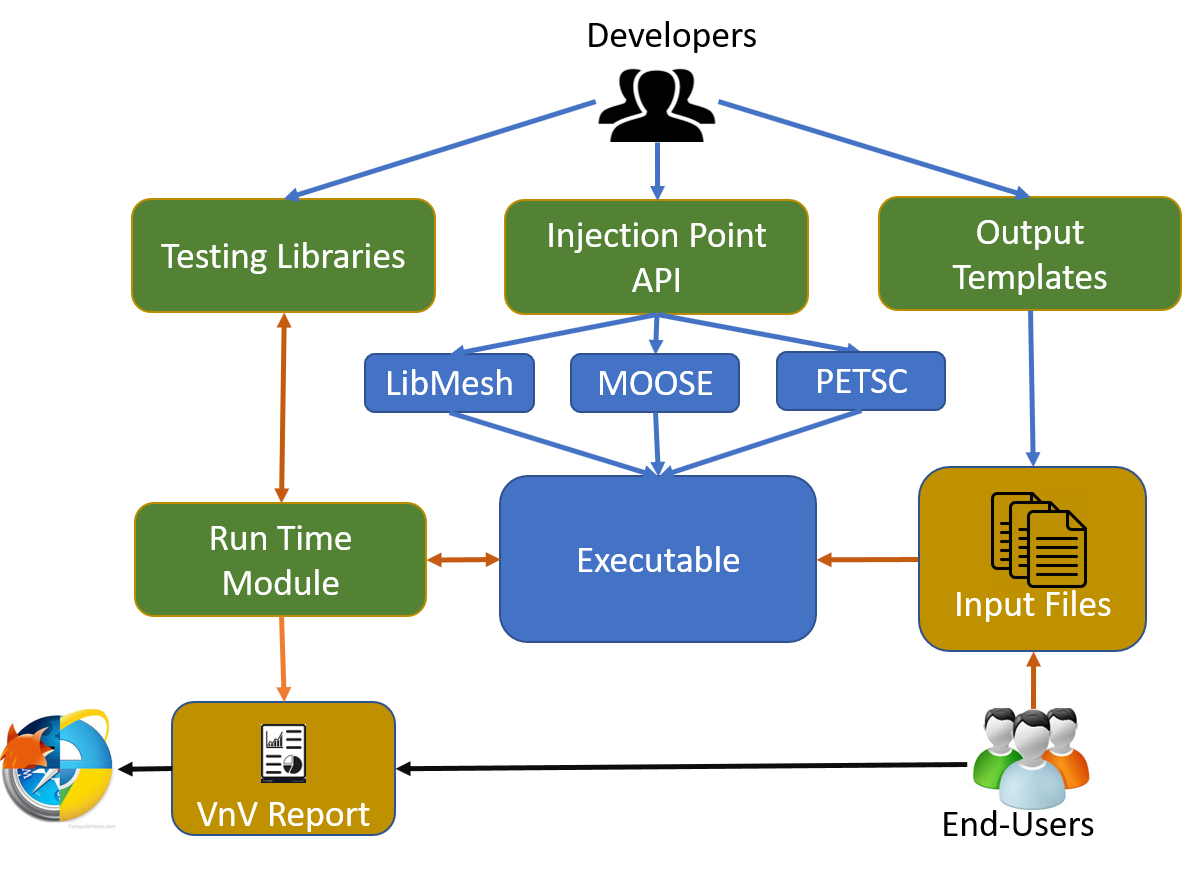
\includegraphics[width=0.7\textwidth]{./narrative/figures/VnVOut.png}
 \caption{ The VnV toolkit. Here, green boxes represent core functionalities. Developer interactions are shown in blue, runtime interactions are shown in orange and post-processing interactions are shown in black. \label{fig:toolchain} } 
\end{figure}
 
Figure~\ref{fig:toolchain} uses the MOOSE tool-chain to show how developers and end-users will interact with the VnV framework. The first step is to define the injection points. These injection points will be placed at key locations of the code where testing can and should take place. Developers will also complete an output template describes the state of the simulation at each injection point. That specification will be used to populate the final VnV report. 

The next step is to create a VnV test. The tests are developed in external libraries and hence, can be developed either by the developer of the simulation, or by the end-user of the code. The core framework will also include a robust set of general purpose \VV tests. Each test will be accompanied for a Markdown formatted template file. Like injection points, this markdown file will be used to
describe the test and present the results. The VnV framework supports a custom markdown format that includes a range of data visualization techniques. We envision that the developers of a numerical simulation package will ship the library with hard-coded injection points and a set of custom \VV tests. 

End-users will be able to generate a customized input configuration file for each executable. This configuration file will contain information about every injection point located in the call-graph of the simulation; including those in external 3rd party libraries. After customizing that file, generating a VnV report is as simple as running the simulation.
 
In summary, once integrated into an application, the VnV framework will provide a simple mechanism for creating self verifying, self describing, explainable numerical simulations. This will significantly reduce the burden associated with \VV for end users, thereby increasing the usability of the tools for non-expert end-users. The core functionality of the VnV toolkit will be released as open source for use in academic and enterprise applications, with RNET providing commercial support, training and integration contracts to interested parties. A commercial license will be required to incorporate the VnV toolkit into for-profit applications;


\subsection{Anticipated Public Benefits}
Numerical modeling and simulation (M\&S) is extensively used in numerous scientific and engineering fields and disciplines such as computational fluid dynamics, high energy physics, nuclear engineering, and computational finance. The prevalence of smaller scale finite element analysis (FEA) software is even wider, with applications ranging from design optimization in \$10 polycarbonate trinkets up to large scale parameter optimization of fighter jet wings. In all cases, the software used to inform the designs of these products must be verified and validated; and in all cases, the verification and validation of this software is a complex, time consuming task requiring input from experts across the broad spectrum of numerical simulation specialty areas (i.e., linear solvers, nonlinear solvers, finite element methods, physical domain specification, data analysis, etc.). 

While most high quality simulation packages have robust internal V\&V regimens, few (if any) ship with a functionality that streamlines end-user \VV. Instead, software simulation developers often take a legal approach, whereby the licensee include language to the effect of ?use at your own risk? or ?this software is released as-is, with no guarantee it is fit for the intended purpose?. The VnV toolkit tool addresses the need for simple end-user validation in numerical simulation codes by providing a unified framework that facilitates the development of explainable numerical simulations. These explainable simulations provide the end user with not only the result, but also a detailed report on how the solution was obtained and the reasons it should be trusted. This detailed report does not shift the burden of end-user \VV to the developer, that is, and always will be the responsibility of the end-user; rather, the framework provides a mechanism for providing the end-user with a level of knowledge about the inner workings of the simulation far beyond what is provided in most numerical simulation tools. 

The VnV toolkit capitalizes on a growing need for tools that facilitate the V\&V of simulations designed by the end-users of highly configurable numerical simulation packages. End-user V\&V is extremely important because the ultimate costs of a design failure (e.g., financial, injury, or loss of life) lies with the simulation software user; any attempt to shift the blame to the software developers of simulation library X (including the V\&V toolkit) will certainly fall on deaf ears. 

End-User V\&V is essential, expense to setup and maintain, and supporting end-user V\&V is difficult. Undetected errors in numerical simulations propagate into physical designs creating issues that can cost millions of dollars to fix, cause catastrophic damage to the environment, and, in the worst case scenarios, result in the loss of human life. The Sleipner platform accident \cite{jakobsen1994sleipner,collins1997failure} is a prime example of the potential problem, an offshore platform collapsed due to failures in the finite element simulation with devastating consequences (and \$700M in damage). The Sleipner accident demonstrates how a poorly verified numerical simulations can significant consequences on business, the environment, and society.

Benefits of the VnV framework include; explainable numerical simulations that increase trust in the solution (VnV enabled simulations produce both a traditional result and a description of how the solution was obtained and why it can be trusted), runtime V\&V configuration (reduces setup time and allows the users of the code to iteratively build a robust \VV regimen without ever touching the source code of the simulation), a robust collection of V\&V tools (improves efficiency by providing statistical assertions optimized for performance in a large scale distributed settings), automated production grade documentation generation (reduces time to market and reduces the burden of meeting the \VV reporting requirements), and cross-library support (multilingual, cross library V\&V testing provides a simple mechanism for facilitating end-user V\&V at all levels of the simulation hierarchy). While focusing no end-user V\&V, the features provided by the VnV framework benefits both simulation developers (our customers) and end-users (users of the simulation software). 

The customers of the VnV framework include the commercial and government entities that develop large-scale numerical models and simulations (e.g., ORNL, Idaho National Laboratory, AFRL, ANSYS, CD-adapco, universities). For developers, integrating support for end-user verification is also an expensive, time consuming task.  By allowing the developer to focus on their area of expertise, these third party packages dramatically reduce the time to market. However, robust end-user \VV requires through testing at every level of the simulation hierarchy, and as such, requires the developer to fully understand and modify the third party simulations. Such requirements counteract the primary benefit of using the third party libraries, knowledge compartmentalization, and as such, make supporting end-user \VV an unenviable task.  RNET will provide training, support, and integration services to integrate the VnV framework into new and existing code bases, as well as contract based services for extending the toolkit to fit specific needs. For these customers, the benefits include streamlining their internal \VV practices, and an increase in the usability, reliability and confidence in their final product. Additionally, including end-user \VV features into their products will provide a differentiating feature to their end-users. 

The true beneficiaries of the \VV framework are the end users of the advanced numerical simulation products. By removing the burden associated with \VV, the VnV framework will ensure erroneous errors do not propagate into final designs. All in all, the VnV framework will afford researchers and engineers with the knowledge required to drive the next generation of technological advancements. 

\subsection{Phase I and Feasibility Demonstration}

The goal of the Phase I effort was to demonstrate the feasibility of a framework that facilitates end-user solution
verification in advanced numerical simulation. To that end, the project team spent the majority of the Phase I
project developing a prototype of the VnV toolkit.

\subsubsection{The VnV Injection Point System}

The injection point system was written in C++ with a focus on minimizing the amount of 
code needed to insert injection points into existing code bases. 

\begin{figure}
 \centering
 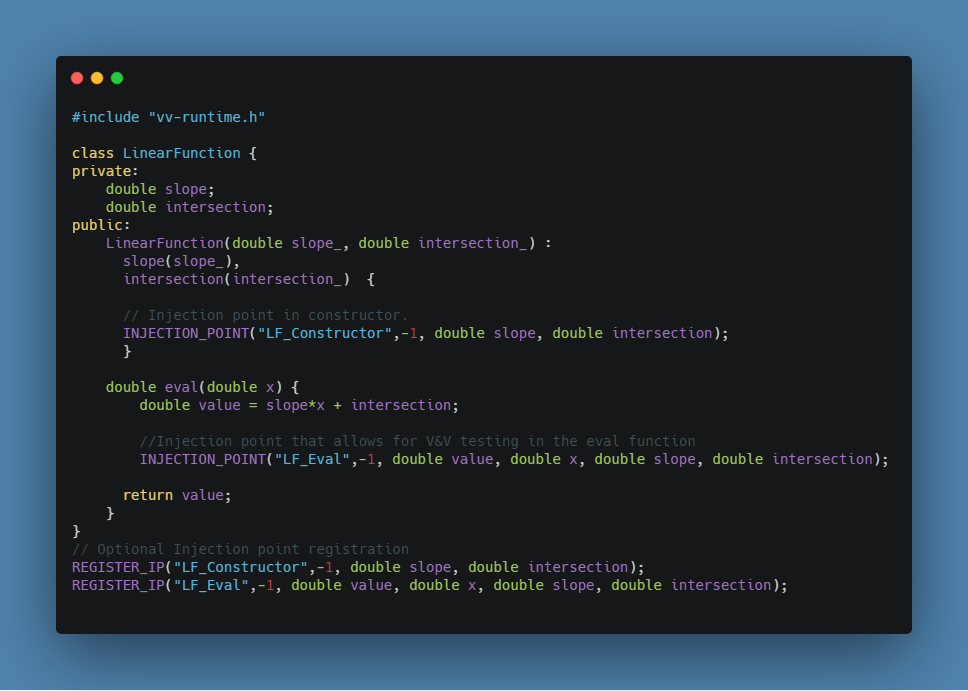
\includegraphics[width=1.0\textwidth]{./narrative/figures/code-example.png}
 \caption{Example of a single stage injection point in a C++ member function. \label{fig:example}}
\end{figure}

Integrating of an injection point into an existing code is a two step process; (1) include the header file, (2) place injection point in the code and (3) register the injection point. Figure~\ref{fig:example} shows a function that has been augmented with a single stage injection point. 

Developers will insert injection points using the INJECTION\_POINT macro. The format for this macro is:

\begin{verbatim} 
INJECTION_POINT( <name>, <stage>, <type> <variable>, ...)
\end{verbatim}

Here, ``name'' is the id that will be used to define the injection point in the configuration files and the final reports. This name must be unique across all injection points in an executable. The stage parameter is an integer value that defines the step that this injection point belongs to. Using this parameter, the developer can set up multi-staged injection point testing. This allows for data collection across multiple code locations. 

The developer defines the variables available for inspection using the variable parameter. During preprocessing, the macro expands this variable definition as 
\begin{verbatim}
 <type> <variable> --> "type", (void*) &variable 
\end{verbatim}

At runtime, the VnV injection point factory compares the ``type'' of each variable against the type of variables supported by each 
VnV test. When a match is found, the framework casts the void* pointer back to its correct type and forwards it to the test for processing. There are several risks associated with this approach, the most important of which is the memory corruption the could occur from a bad cast. Addressing these issues is a major goal of the the Phase II project (see Section~\ref{sec:workplan}).

The final step in the creation of an injection point is to write the output template. This template is used to populate 
the final VnV report. The output template is a YAML file containing a markdown formatted description of the injection point. There is 
no requirement that a output template be supplied, however, the more information that can be provided, the more informative the final VnV report will be. The VnV framework supports a custom markdown format that includes a number of data visualization extensions (2D charts, 3D visualization, Tables, latex, etc). Most importantly, the custom markdown format provides a mechanism for automated post-processing of the data collected during VnV testing. 

\subsubsection{The VnV Testing Interface}

The second facet of the injection point system are the \VV tests. The test interface was developed under the assumption that tests should be loaded at runtime and defined independently of the source code. As such, the test interface was built using a C++ plugin pattern. 

The framework includes a library generation script that will automatically build the directory structure and makefiles required to 
build a testing library. Once the library has been initialized, the user can begin to develop individual tests. 

To assist in the development of tests, and to avoid issues with incorrect type-casting, a test generation script is also included. This script automatically generates the boiler plate code required to implement the testing interface while also taking care of the required typecasting. With this, implementing a custom test requires the developer to:

\begin{itemize}
 \item {\bf Implement the ``declareParameters'' function}. This function defines the parameters required to perform
 the test. For example, the test in Figure~\ref{TODO} requires two doubles; one called slope and the other called intersect. The user will map the injection point variables to the test variables using the test configuration file. 
 \item {\bf Implement the ``runTests'' function}. The variables passed to the test are direct pointers to the variables in the code. Hence, tests should not modify the pointers in any way; however, the phase I prototype does not strictly enforce this requirement. Beyond that requirement, there is not limit on the procedures that can be run inside a test. All data required for post-processing should be output inside this function using the supplied ADIOS engine. 
 \item {\bf Write the output template.} Like injection points, all tests should be accompanied by a output template. The output can be used to automatically post-process and visualize the data collected during each test. 
\end{itemize}


\begin{figure}
 \centering
 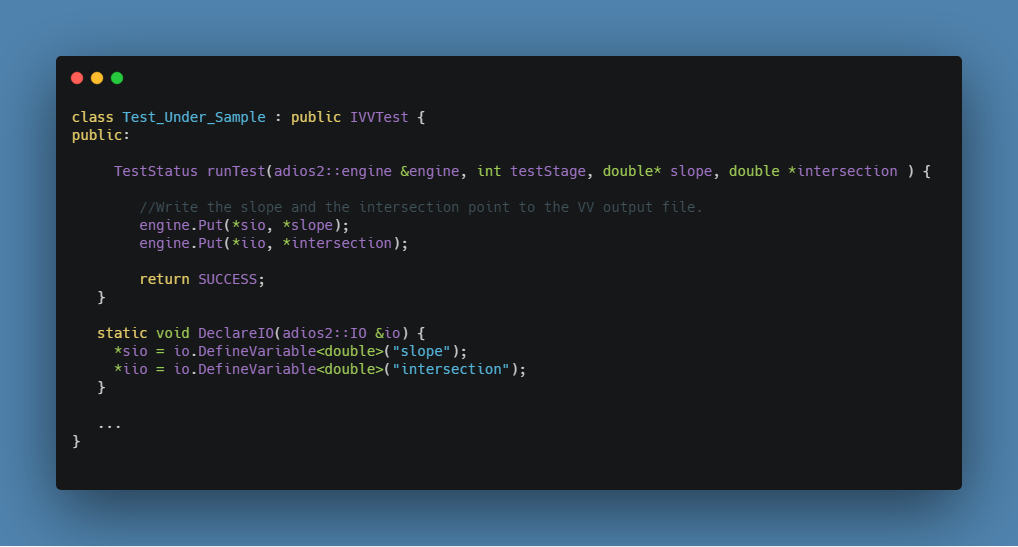
\includegraphics[width=0.95\textwidth]{./narrative/figures/testcode-example.png}
 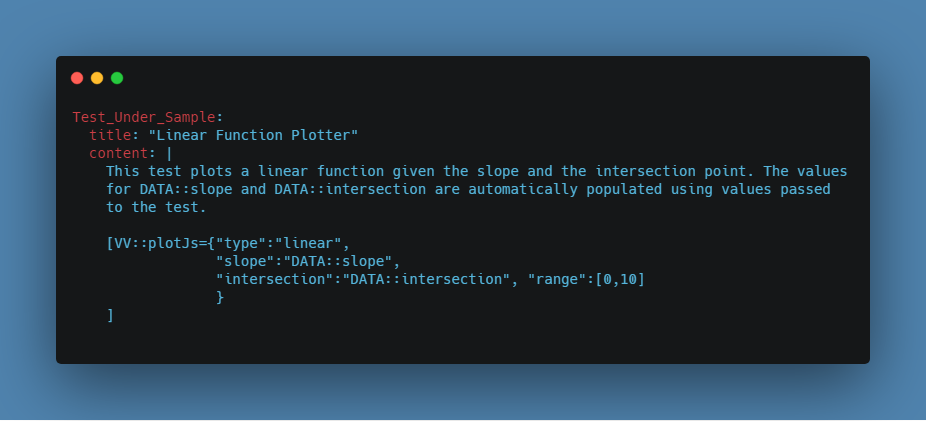
\includegraphics[width=0.95\textwidth]{./narrative/figures/test-example.png} 
 \caption{Sample code a custom VnV test for tracking the slope and intersection point of a linear function. \label{fig:test-example}}
\end{figure}

\subsubsection{The Runtime Module}

Once the injection points have been declared and the tests created, the next step is to develop the XML test configuration file. Using this XML file, users can configure which testing libraries to load and which tests to run. The test configuration file is used to map injection point parameters to test parameters. For example, Figure~\ref{TODO} shows a portion of a test configuration file that inserts the LinearTest function shown in Figure~\ref{TODO} into the ``IP\_1'' injection point defined in Figure~\ref{TODO}. Please see the final report for a full description of the XML format supported by the phase I prototype.

Turning on VnV testing across all libraries linked to the executable is as simple as calling an initialization function with a valid input configuration file.

\subsubsection{Automated Report Generation}

The final step in the VnV pipeline is the automatic report generation. At the core of the report generation system is a custom markdown extension. This extension supports a range of custom data visualization features that interact directly with the output data in the ADIOS2 output file. For example, users can specify markdown that renders as an interactive 2D visualization automatically populated with data obtained during VnV testing (the line chart shown in  Figure~\ref{rendered-example} is generated using this functionality). Other features include 3D visualization using VTK.js and search-able tables with tabular.js. The extension also includes support for running custom python scripts during compilation. This allows for infinite possibilities with regard to processing the test outputs. For example, a user can write markdown that, during compilation, runs a paraview script and then display the results using the VTK.js.   

Figure~\ref{rendered-example} shows a screen-shot of a VnV report generated using this approach. The main layout consists of two components; the index and the content. The index in generated directly from the VnV output file. Each entry in the index represents an injection point that was reached during the execution of the simulation. The content section is generated automatically from the YAML specification files. In this case, the user has completed a test titled ``Linear Function Plotter'' inside an injection point called ``Linear Function Constructor''.  

\begin{figure}
 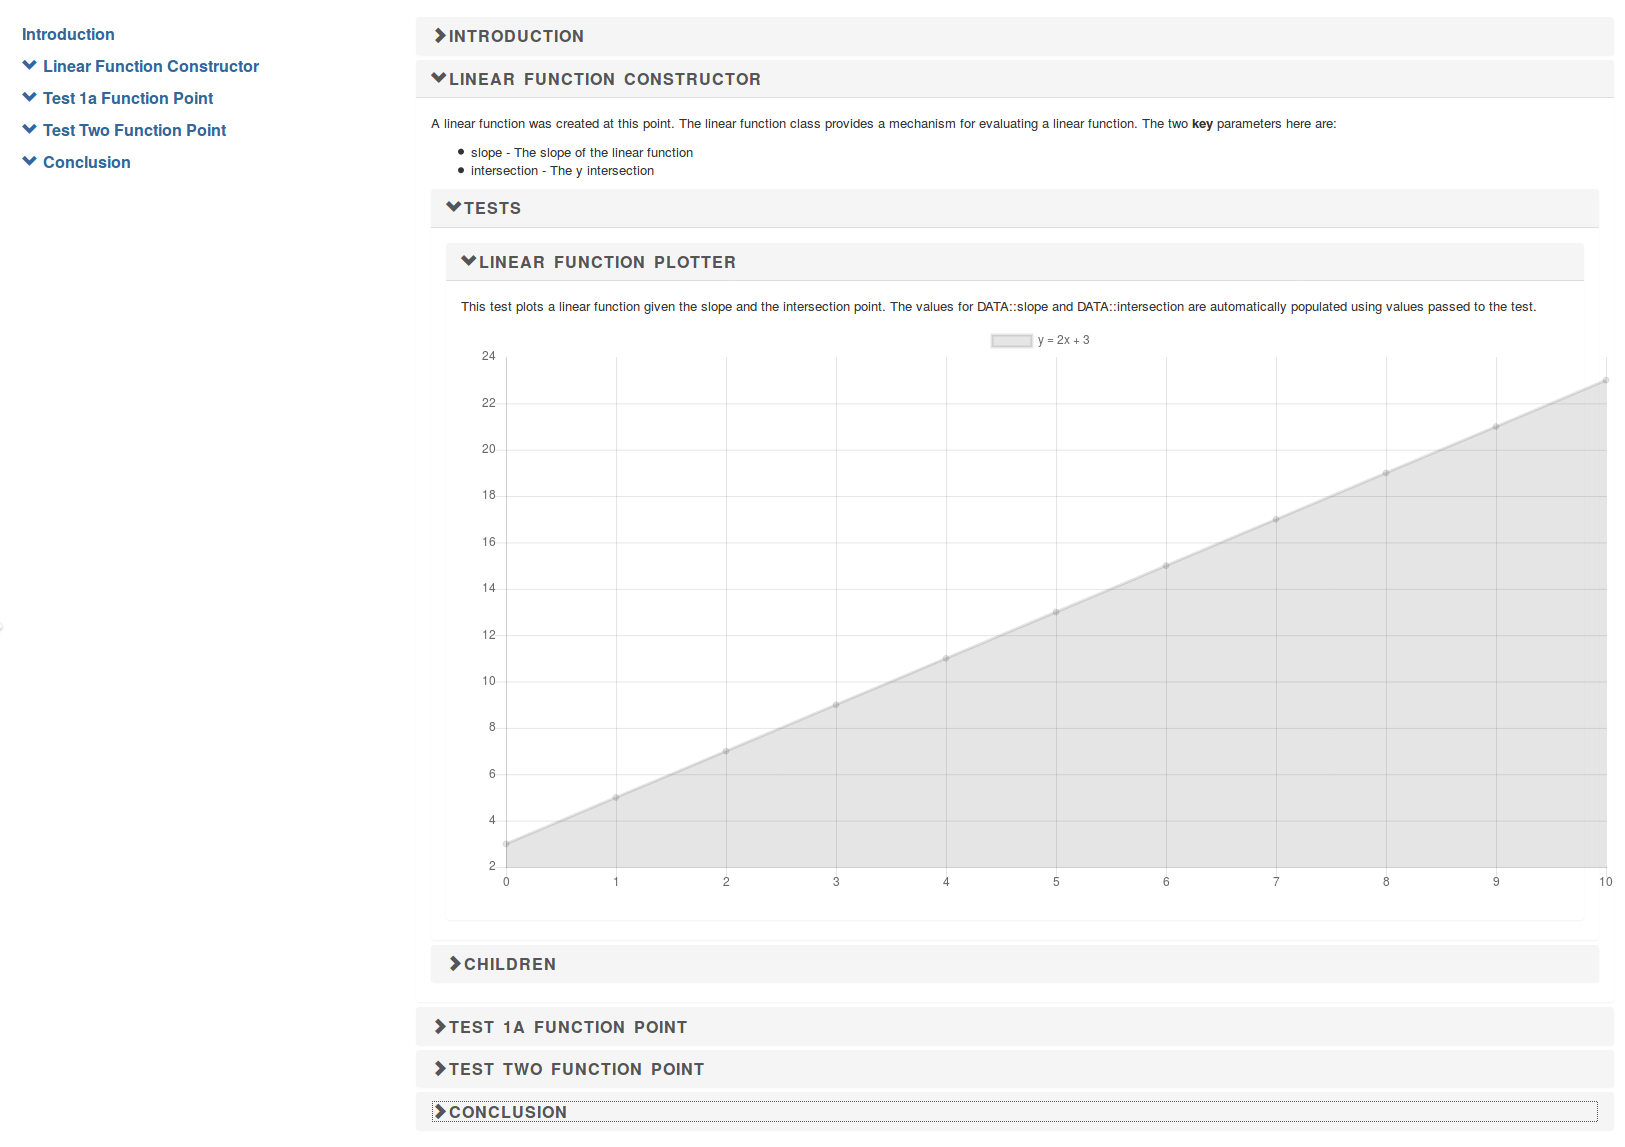
\includegraphics[width=\textwidth]{./narrative/figures/render-example.PNG}
\caption{ An example of the VnV report generated automatically from the VnV output files and the injection point and test specification files. \label{rendered-example}}
\end{figure}
 
The key point to note here is that this interface was generated automatically from the VnV output file.

In summary, during Phase I, the project team created a functioning prototype of the VnV framework that provides:
\begin{itemize}
 \item A clean mechanism for inserting injection points in existing codes
 \item A simple interface for defining custom tests 
 \item A report generation system that automatically creates an interactive server-less web report based on the VnV output.
\end{itemize}

As will be described in the workplan, the goal of the Phase II project will be to take this initial prototype and extend, harden and 
optimize it for use in high performance computing applications. 





























